% Introduction chapter to the topic

\chapter{Introduction}
\label{ch:intro}

This chapter will give a justification for the Persuasive Electric Vehicle (PEV) project. For that, the 3 main topics that caused this idea to flourish will be discussed, including their weak points and how PEV tackles them. These topics are: cities, autonomous vehicles and shared mobility. 

\section{The future of cities}

In the coming decades, it is expected that population in urban areas will grow from 50\% to 70\% \citeintro{Shahrokni2014c}. Furthermore, 95\% of that expansion will happen in developing countries \citeintro{Salvini2018g}. As a result of this migration important social and environmental challenges will arise such as fuel production, air pollution, waste management, urban transportation \citeintro{Girardet2008b}, etc.

To this day, cities are dealing with deeply concerning issues regarding transportation that will only get worse with the rapid growth it is expected in the next years \citeintro{Mikoajczyk2017, Zavitsas2010}:

\begin{itemize}

  \item \textbf{Traffic congestion}: The number of private cars added to the amount of trucks, vans, taxis, buxes and rest of vehicles have lead to gridlocks in major cities across the globe. This causes increased traffic pollution, longer commutes and higher tensions among drivers.

  \item \textbf{Sprawling cities}: The rapid growth of cities has pushed people to the outskirts due to an exponential increase in the housing price. Therefore commutes become longer and transportation networks grow more complex.

  \item \textbf{Parking}: Parking is a major issue due to the amount of space it occupies, thus increasing the already high land demand inside urban environments.

\end{itemize}  

Over the last decades, the term 'Smart City' has become more popular to describe cities that make investments in novel infrastructures and Information and Communication Technologies (ICTs) \citeintro{Shahrokni2014c}. The purpose for this trend is to accelerate economic growth while managing resources more efficiently, being one of those resources transportation \citeintro{Caragliu2011b}.

Among the various solutions that have been proposed to improve mobility infrastructure, 2 of them will be discussed due to their close link to the main topic of this thesis: \textbf{Autonomous Vehicles} and \textbf{Bicycle Sharing}.

\section{Autonomous Vehicles. Future of transportation?}

The field of Robotics has gained a great deal of traction in the last years, whether it is for the field of biomedicine, construction or Artificial Intelligence \citeintro{Yang2018a}. And the field of Autonomous Vehicles (AVs) has followed this trend. 

AVs, once utopy, are becoming every passing year a real possibility in the not-so-far future \citeintro{Wired2018}. Apart from big names such as Google's Waymo, Tesla, Uber, Lyft or Nvidia, this decade has seen the surge of smaller companies dedicated to developing self-driving car technologies. The latter group is where companies like \href{https://www.nutonomy.com/}{NuTonomy} and \href{https://www.optimusride.com/}{Optimus Ride} belong. \autoref{fig:auton_vehic} shows some examples of these vehicles.

\begin{figure}[htb]
  \myfloatalign
  \subfloat[Google's Waymo spinoff company]
  {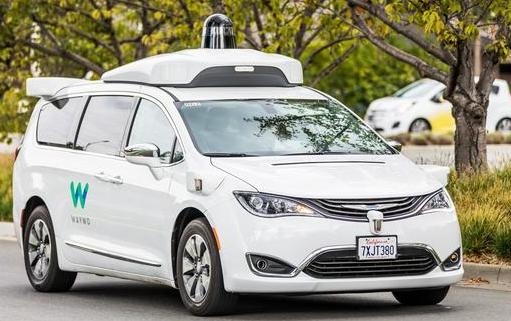
\includegraphics[width=.45\linewidth]{pictures/01/waymo}} \quad
  \subfloat[Tesla's Autopilot]
  {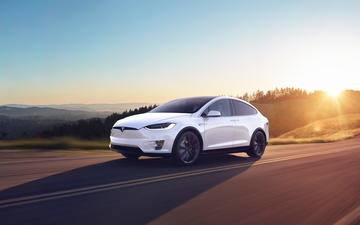
\includegraphics[width=.45\linewidth]{pictures/01/modelx}} \\
  \subfloat[Nutonomy's AV]
  {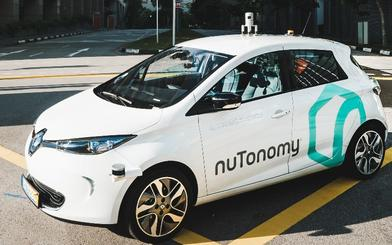
\includegraphics[width=.45\linewidth]{pictures/01/nutonomy}} \quad
  \subfloat[Optimus Ride's autobus]
  {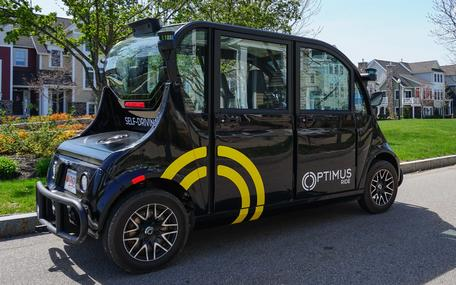
\includegraphics[width=.45\linewidth]{pictures/01/optimus}} 
  \caption[Current state of AVs]{Current state of AVs}
  \label{fig:auton_vehic}
\end{figure}

\subsection{Some history on Self-Driving Vehicles}

First attempts to build robotic vehicles date as early as 1920s \citeintro{Bimbraw2015} when the first radio controlled vehicles were designed. In the decade of 1980, there were serious attempts at building autonomous vehicles, such as the following projects:

\begin{itemize}

  \item \textbf{Prometheus} (Program for a European Traffic with Highest Efficiency and Unprecedented Safety) project: The aim of this project was to build a civilian car to navigate on highways or cities (\ie more structured environments) \citeintro{Xie1993, Flyte1995}. The vehicle chosen was a Mercedes-Benz van designed by Ernst Dickmanns and during test drives on highways it achieved a maximum speed of 96 km/h and drove for about 20 km\footnote{History on the car: \url{https://www.mbscottsdale.com/blog/mercedes-benz-whensday-the-prometheus-project/}}.

  \item \textbf{ALV} (Autonomous Land Vehicle) project: This project was developed by DARPA in America (Prometheus was from Europe) in collaboration with Carnegie Mellon University. The van employed was able to navigate, plan routes and avoid obstacles in coarser terrains than the Prometheus van for 5 km and at a speed of 20 km/h \citeintro{Leighty1986, Goto1987}. 
\end{itemize}

Both cars are shown in \autoref{fig:1980}.

\begin{figure}[htb]
  \centering
  \subfloat[Prometheus van]{
    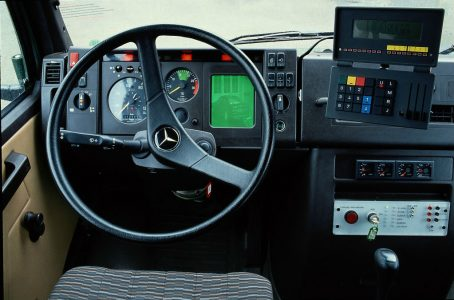
\includegraphics[width=.45\linewidth]{pictures/01/prometeus}
  } \quad
  \subfloat[DARPA's Autonomous Land Vehicle] {
  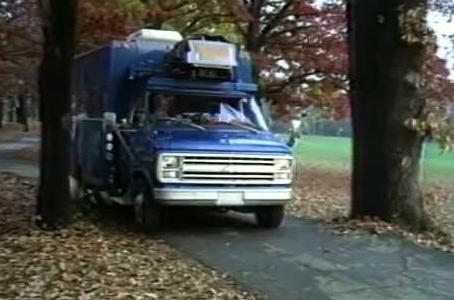
\includegraphics[width=.45\linewidth]{pictures/01/navlab}
  }
  \caption{The first serious attempts to build AVs}
  \label{fig:1980}
\end{figure}

In 2003, DARPA launched the Grand Challenge \footnote{\url{http://archive.darpa.mil/grandchallenge/}} to promote the development of unmanned vehicles. The Challenge was to drive a car autonomously through an unknown off-road terrain. More specifically, a 142 mile-long course across the Mojave desert in less than 10 hours \citeintro{Thrun2006} \citeintro{Seetharaman2006}. There were 107 teams registered, 15 of which made it to the race, although none of the participants drove further than 5\% of the total length. In 2005, the challenge was repeated and 5 teams managed to finish the race out of 197. Stanford University won that race with a car named Stanley (\autoref{fig:stanley}).

\begin{figure}[htb]
  \centering
  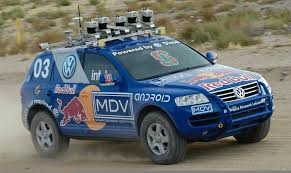
\includegraphics[width=.9\linewidth]{pictures/01/stanley2}
  \caption{DARPA Grand Challenge's first winner: STANLEY}
  \label{fig:stanley}
\end{figure} 

In 2009, Google launched the Self-Driving Car project that became a company named \href{https://waymo.com/}{Waymo}. Since its inception, this project has achieved very interesting milestones and it is the company that has driven more miles autonomously by far \citeintro{Hook2018}.

\subsection{Current state of autonomous driving and levels of autonomy}

Nowadays, virtually almost every car has some sort technology embedded in it, that provides it with a certain level of autonomy or 'intelligence'\citeintro{Litman2014}. Examples of these advancements are \citeintro{Thompson2017}:

\begin{itemize}

  \item \textbf{Self-parking}: A couple years ago, automakers like \href{https://www.toyota-europe.com/world-of-toyota/safety-technology/parking-aids}{Toyota}, \href{https://www.mbusa.com/mercedes/technology/videos/detail/class-SL_Class/title-convenience/videoId-bef758b451127410VgnVCM100000ccec1e35RCRD}{Mercedes} or \href{https://www.bmw.co.uk/bmw-ownership/connecteddrive/driver-assistance/intelligent-parking}{BMW} started developing cars that could find parking spots and maneuver the car to eventually fit it in. These technologies generally rely on ultrasonic sensors and cameras, taking into account cars' movement restrictions \citeintro{Paromtchik1996} (it will be explained in \autoref{ch:concepts}).

  \item \textbf{Automatic emergency-braking}: It detects imminent crashes and attempts to minimize the impact of them. These technology alerts the driver first with visual or sound warnings and if there is no response, the vehicle stops immediately.

  \item \textbf{Semi-autonomous drive system}: There are already cars on the market that can drive themselves autonomously on highway conditions. This is the case of \href{https://www.tesla.com/autopilot?redirect=no}{Tesla's Autopilot} or \href{https://media.gm.com/media/us/en/cadillac/news.detail.html/content/Pages/news/us/en/2017/apr/0410-supercruise.html}{Cadillac's Super Cruise}. These systems are capable of adapting to traffic conditions on highways and even steering on more complicated roads, but they still require the driver to pay attention to the road.

\end{itemize}

According to the Society of Automotive Engineers (SAE), there are 6 levels of automation\citeintro{SAE2015} as show on \autoref{fig:sae}.

\begin{figure}[htb]
  \myfloatalign
  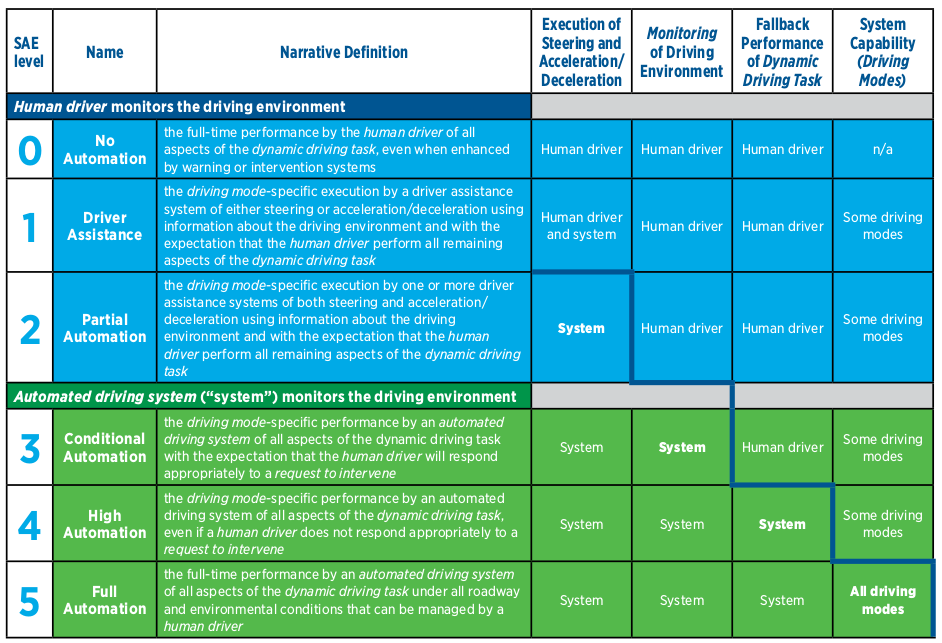
\includegraphics[width=\linewidth]{pictures/01/sae}
  \caption{Levels of Autonomy according to SAE}
  \label{fig:sae}
\end{figure} 

The first 3 levels (from 0 to 2) is where most cars lie nowadays, specially levels 1 and 2 thanks to the advances mentioned above. That means humans are still in charge of monitoring the environment. Tesla's Autopilot lies on level 3 though under certain conditions but it is still under development after the deadly crash in 2016 \citeintro{Hawkins2017}. With regards to level 4 autonomy (in other words, car is able to full self-drive but under certain road and weather conditions), Uber and Waymo announced plans to test driverless taxis last November \citeintro{Bergen2017, Lee2017}. 

Nevertheless, level 5 autonomous cars seem to be still a distant possibility. According to SAE (\autoref{fig:sae}), level 5 implies that no human intervention would be needed in any condition and that is not the case today, since AVs cannot be operated under heavy rain or snow conditions, unpaved roads or with diverse traffic \citeintro{Simonite2016}.

\subsection{Advantages of AVs}

The rise of self-driving cars and related technologies is not a product of coincidence rather than the general belief among scientists and industry that they will bring many benefits in terms of safety, productivity and wealth \citeintro{Litman2014}. In the following paragraphs, some of these advantages will be discussed.

\parunder{Road safety} According to the World Health Organization (WHO), every year around 1.25 million people lose their lives in car accidents and 20-50 million people get injured \citeintro{WHO2018}. In the United States human caused car accidents account for 90\% of the crashes \citeintro{Fagnant2015, UsDep2008}. By adopting AVs in large scales, distractions will happen less frequently, therefore reducing the number of deadly accidents.

\parunder{Improved mobility} The daily commute is one of the tasks AVs could help many drivers with. On average, it takes 26 minutes \citeintro{Uhlemann2016a} to go from home to work and back, time that could be spent doing more productive or rewarding tasks. Self-driving vehicles could be transformed into mobile bedrooms, playgrounds or offices to suit the demand of their users [citation], as it is Mercedes' self-driving concept car shows for example (\autoref{fig:mercedes})\footnote{https://www.youtube.com/watch?v=8aEWHdduPwc}.

\begin{figure}[htb]
  \myfloatalign
  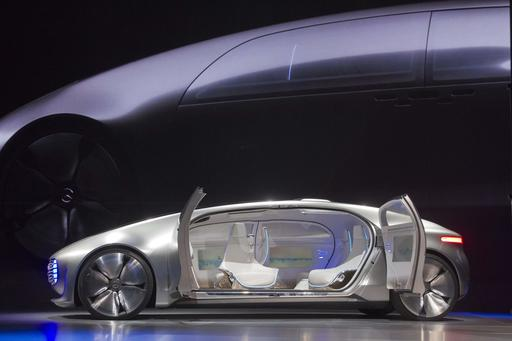
\includegraphics[width=\linewidth]{pictures/01/mercedes}
  \caption[Mercedes self-driving car]{Mercedes self-driving car}
  \label{fig:mercedes}
\end{figure} 

\parunder{Better Traffic Flow} Some researchers have shown that AVs can improve traffic flow \citeintro{Talebpour2016}. Since self-driving cars might be able to connect to other cars and features of the environment, and have lower response times, they can: 
\begin{enumerate} 
  \item Anticipate events faster and allow for smoother braking and acceleration.
  \item Use lanes and intersections more effectively by reducing gaps and platooning (\autoref{fig:platoon}).
\end{enumerate}

\begin{figure}[htb]
  \centering
  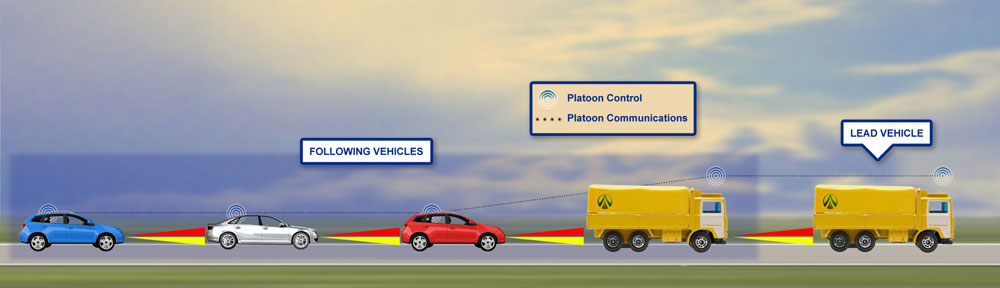
\includegraphics[width=\linewidth]{pictures/01/platoon}
  \caption{Platooning representation on a highway}
  \label{fig:platoon}
\end{figure}

\parunder{Shared Networks} One of the key attactives for AV technology is that it could enable new travelling modes (combining provate and public) such as communally-owned shared vehicles \citeintro{Haboucha2017}. Shared Autonomous Vehicles (SAVs) might potentially benefit the environment by reducing the need for car ownership and parking \citeintro{Fagnant2014a}. Users with similar destinations could share rides (in the same manner as with current carsharing services). However, the main advantage over what is available today, is that after the ride they could autonomously relocate themselves to more demanded areas, thus reducing the need for parking lots that could be transformed in green areas \citeintro{Litman2014}. 

\subsection{Disadvantages of AVs}

Even though self-driving technology has a vast potential to improve many aspects of society, it is not perfect and it raises concerns among researchers, policy makers and general public. Many of the positive aspects described above have their negative counterparts as it will be discussed in the next paragraphs.

\parunder{High costs} Even though costs could be reduced due to car reduction, the technology needed to transform a regular car into a self-driving one increases the prize dramatically. Each of the Light Detection and Ranging (LIDAR) sensors installed can cost between 30.000\$ and 85.000\$ \citeintro{Shchetko2014a} which makes AVs unaffordable for the vast majority of the population.  

\parunder{Liability and ethical questions} As AVs become more pervasive in everyday landscape, questions will arise when these vehicles are involved in any type of accident \citeintro{Fagnant2015}. When car's software fails, who is to blame: the software engineer, the company? How can an insurance company be convinced of the reliability of self-driving vehicles?

Moreover, if a crash is inevitable and the car has to decide between 2 evils, how can it make the decision? These ethical questions pose a major challenge when it comes to real world implementations and there is no clear answer. From MIT Media Lab's group \href{https://www.media.mit.edu/groups/scalable-cooperation/overview/}{Scalable Cooperation}, an initiative called Moral Machine \citeintro{Rahwan2016} was launched in order to create a discussion on these moral dilemmas and build a 'crowd-sourced' image of how intelligent machines should behave\footnote{A test can be taken with different scenarios: http://moralmachine.mit.edu/}.

\parunder{Public perception} Another issue to overcome is public perception. First of all, because when self-driving car technology reaches the mass market, professional drivers might start losing their jobs \citeintro{Litman2014}. Trust on the technology is an important obstacle to overcome, since few people will feel uncomfortable at first, being the technology new and not sufficiently tested \citeintro{Howard2014, Bansal2017}. 

\parunder{Safety and Security} Electronic security is a major concern for every major car- and policymaker, and for the general public \citeintro{Schoettle2014}. Hackers, terrorist groups or employees could target the intelligent system of the vehicles and cause major disruptions on the whole network \citeintro{Fagnant2015}, by forcing cars to collide or exposing users' locations.

\subsection{When will AVs hit the road?}

Due to these challenges and many other that arise when developing self-driving technologies, experts believe level 4 and 5 AVs will not be available to the general public until the 2040s--2050s \citeintro{Litman2014, Rowe2015}. 

\section{Shared mobility}

Shared mobility has already been mentioned as a future field of application of AVs, but the growth it has undergone in past years by itself is worth noting, since it has crutial implications for the future of transport in cities.

Many car sharing companies have already achieved a great market share like \href{https://www.zipcar.com/}{Zipcar}, \href{https://www.car2go.com/ES/en/}{Car2Go}, or even \href{https://www.uber.com/en-ES/ride/uberpool/}{Uber}'s latest services. However, this section will focus on bicycle sharing systems, due to their applications and benefits for cities across the world.

\subsection{What is bicycle sharing?}

Bicycle sharing or bikesharing corresponds to the public shared use of bicycle fleets that has gained attention these past years \citeintro{DeMaio2009, Shaheen2010} in many regions of the world such as Europe, US and China.

The case of China is specially striking, since many bikesharing startups have sprung out in the past years, and the biggest companies among those, \href{https://www.ofo.com/es/en}{Ofo} and \href{https://mobike.com/global/}{Mobike}, already have 19 million bikes across the world \citeintro{Yang2018}.

Nevertheless, bicycle sharing it is not a radically new concept from this century. In fact, its origins trace back to the 1960s and there have 3 generations in bikesharing history \citeintro{DeMaio2009}:

\begin{itemize}

  \item The first generation started in 1965 and the concept was to provide with ordinary bikes that could be parked anywhere. However, bikes were vandalized very often.

  \item Second generation was born in 1993, when bikes had to be parked on specific docks or stations. Although it improved the previous versions, bicycles were still subject to theft due to user anonimity.

  \item Third generation (the current one) bikes already incoporate smart technologies like electronic locks or bicycle tracking to improve security.

\end{itemize}

The rise of this transportation method is not casual since it comes as an answer to 3 key aspects in cities \citeintro{DeMaio2009}:

\begin{itemize}

  \item \textbf{Increased cycle usage}: This way healthier lifestyles are promoted in urban environments.

  \item \textbf{Increase first/last mile connection}: Bike sharing can provide its users with connection from their homes/working areas to other means of transport such as buses, trains or subway. Moreover, bike fleets can be used to tranport not only people but packages and other goods across the city, thus avoiding traffic congestions caused by larger vans or trucks.

  \item \textbf{Reduce environmental impacts}: Biking is an emission--free means of transport and therefore it can help mitigate common concerns in cities like global climate change, energy supply or varying fuel prices \citeintro{Shaheen2010}.

\end{itemize} 

\subsection{What are the current disadvantages of these approaches?}

Again there is no perfect solution to urban transportation and bicycle sharing suffers essentially from 2 issues.

\paragraph{System rebalancing:} The first one, and this occurs to shared automobiles as well, is that they have to be manually relocated in order to guarantee the balance of the system. This implies arranging a logistics network around the city in order to ensure every area they are operated within has a minimum amount of bikes.
  
\paragraph{bike Cemeteries:} Because of these attempts to equilibrate the network, companies must provide with a higher amount of bicycles than necessary and keep higher stocks, all resulting in greater maintenance costs and many times bicycles end up in in landfills. Combining this with market saturation as it is happening in China's markets, 'bike cemeteries' are being formed in the outskirts of cities like Shanghai or Beijing (\autoref{fig:cemetery}) \citeintro{Campbell2018}.

\begin{figure}[htb]
  \centering
  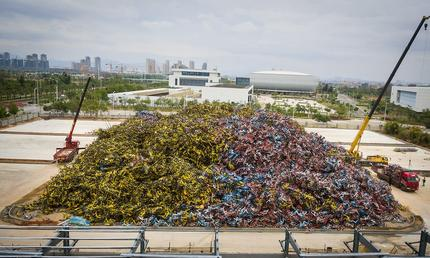
\includegraphics[width=.9\linewidth]{pictures/01/cemetery3}
  \caption[Bike cemeteries outside cities]{Unused bicycles end up forming immense cementeries around cities}
  \label{fig:cemetery}
\end{figure}  

\section{Persuasive Electric Vehicle (PEV)}

\subsection{MIT Media Lab: Home of Innovation}

To understand the PEV project, it is necessary first to put some context on the place of its inception, the Media Lab. According to their website, Media Lab is "an antidisciplinary research lab working to invent the future"\footnote{https://www.media.mit.edu/research/?filter=groups}. In fact it is a place that gathers all sorts of people from various backgrounds such as Arts, Sociology, Computer Science or Engineering and aims at developing ideas that bring technology closer to humans. Since its foundation in 1985, more than 150 companies have spun out of its doors\footnote{https://www.media.mit.edu/about/spin-off-companies/}.

Some of the notable projects are:

\begin{itemize}
  \item \textbf{Scratch programming language}: It is a block-based language initially developed for children but that it is used by people all ages around the world \citeintro{Resnick2009}

  \item \textbf{Harmonix}: Game development company that launched \href{http://www.harmonixmusic.com/}{Rock Band and Guitar Hero}.

  \item \textbf{E-ink}: Company that developed the electronic ink, now used in e-readers around the world \citeintro{Jacobson2003}.
\end{itemize}

\subsection{City Science and its mission}

\href{https://www.media.mit.edu/groups/city-science/overview/}{City Science} is one of the 25 groups of this ecosystem and it is where the PEV is located. The group, led by Professor Kent Larson, is aware of the challeges cities will face in the coming years and is focused on developing platforms and tools that will improve life in cities \citeintro{Larson2012}. There are 3 main research topics at City Science:

\begin{itemize}

  \item \textbf{CityScope}: It is a platform that aims at providing tools for cities and urban planners to model and design infrastructures with the use of simulations and real time data \citeintro{Grignard2018}. The whole system is built around a Lego table, where decision makers can 'play' and see the effects of their solutions in real-time (\autoref{fig:cityscience}).

  \item \textbf{Changing Places}: This group focuses on developing responsive places to live and work in future cities. 2 of the most famous projects are Cityhome which later became the spinoff \href{https://www.orisystems.com/}{Ori} which provides robotic furniture (\autoref{fig:cityscience}), and Escape Pod, a transformable space for either working or resting.

  \item \textbf{Mobility-on-Demand}: This group is focused on efficient shared--use mobility systems and its main project is the aforementioned \textbf{PEV} which will be explained in more detail in the following lines.

\end{itemize}

\begin{figure}[ht]
  \centering
  \subfloat[CityScope]{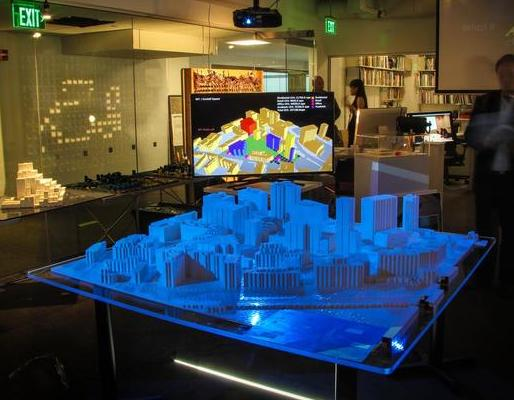
\includegraphics[width=.45\linewidth]{pictures/01/cityscope}} \quad
  \subfloat[Ori system]{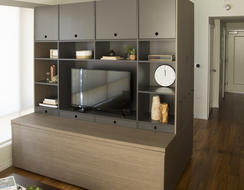
\includegraphics[width=.45\linewidth]{pictures/01/ori}}
  \caption{City Science's CityScope and Ori platforms}
  \label{fig:cityscience}
\end{figure} 

\subsection{Reason for the PEV}

The \href{https://www.media.mit.edu/projects/pev/overview/}{PEV} is an autonomous, lightweight, low--cost, electric and shared tricycle (\autoref{fig:pev}) that aims to be an alternative to both autonomous vehicles and bikesharing systems.

\begin{figure}[htb]
  \centering
  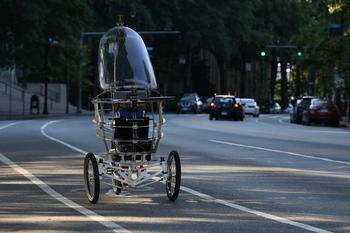
\includegraphics[width=\linewidth]{pictures/01/pev}
  \caption[PEV on the streets]{PEV on the steets of Cambridge, Massachusetts (August 2017)}
  \label{fig:pev}
\end{figure}

The PEV would be operated in 2 different modes:

\begin{itemize}

  \item \textbf{People mover}: People would be able to call a PEV with a phone app (like Uber) and the vehicle would come to the user autonomously. Then the requester would have to ride it to the destination and after the ride, the PEV would leave on its own to another location.

  \item \textbf{Package delivery}: PEV could be used as a package delivery system while user demand is low (for example, at working hours). This way it could help reduce traffic congestion caused in cities by trucks or vans.

\end{itemize}  

It has already been explained taht both AVs and bikesharing systems have their downsides. The idea of the PEV was born to tackle the issues that arise on these approaches as \autoref{tab:avpev} shows.

\begin{table}[htb]
  \centering
  \resizebox{\textwidth}{!}{\begin{tabular}{p{3cm}p{4.5cm}p{4cm}p{4.5cm}}
  \hline
  \multicolumn{1}{c}{\textbf{Aspect}} & \multicolumn{1}{c}{\textbf{AVs}} & \multicolumn{1}{c}{\textbf{Bike Sharing}} & \multicolumn{1}{c}{\textbf{PEV}} \\ \hline
  \textbf{Environmental Impact} & Even though they might reduce traffic, environmental cost will be high & Minimal impact & Slightly bigger (when in autonomous mode) but minimal when riding it \\ \hline
  \textbf{Healthy lifestyle} & They do not promote healthier lifestyles & Cycle usage increases physical activity & Passengers will have to pedal, thus promoting a healthier transport \\ \hline
  \textbf{Infrastructure} & AVs need high-quality roads and special infrastructure that might be costly & They can run on current bike-lanes & It is designed to fit on bike lanes, so it would require less infrastructural support \\ \hline
  \textbf{Road safety} & They are subject to strict regulations due to their risk, so that might slow down their deployment & It is less dangerous so regulation is not as strict & As it it is lightweigth and will operate at low speeds on bike lanes, risk will be lower than with self-driving cars. Therefore deplyoment might be faster \\ \hline
  \textbf{Parking} & They need minimal parking & They need a notable amount of stations & They need minimal parking \\ \hline
  \textbf{Relocation} & They can relocate automatically based on demand & The need to be manually relocated & They can relocate automatically based on demand \\ \hline                                                                                                    
  \end{tabular}}
  \caption[AVs, bikesharing systems and PEV]{Comparison between AVs, bikesharing systems and PEV}
  \label{tab:avpev}
  \end{table}

\section{Thesis Structure}

This thesis is divided as follows:

\begin{itemize}
  \item \textbf{Chapter 2} explores the current technologies available for autonomous vehicles and describes the fundamental elements of the main aspects of self-driving vehicles.

  \item \textbf{Chapter 3} describes the field of Simultaneous Localization and Mapping (SLAM) more thoroughly, as well as providing with the latest approaches.
  
  \item \textbf{Chapter 4} analyzes different slam algorithms applied on a small autonomous robotic platform, that served as a testbed for the PEV.

  \item \textbf{Chapter 5} analyzes the slam approach on the PEV, and what are the best configurations for different scenarios.

  \item \textbf{Chapter 6} shows a simple budget for the project and its timeline.

  \item \textbf{Chapter 7} provides with conclusions on the results obtained on both platforms, improvements that could be tackled and sets the next steps for these vehicles.

\end{itemize} 

